In order to verify the analytical models, we develop an event-driven simulator for shadow replication with CSIM. 
The architecture of the simulator is shown in Fig.~\ref{fig:sim}. The simulator has 5 CSIM processes and they interact
with each other through CSIM events. The first CSIM process is Global Coordinator that launches all other CSIM processes
and output statistics after the simulation is done. Failure Injector is another CSIM process that injects failures to 
the running task instances according to a specified failure distribution. Main and Shadow are two processes that "execute" 
the real-time task. They will run at the frequencies derived from analytical models. Finally, we have a Task coordinator
 that terminates the Shadow process if the Main process finishes, or speed up the Shadow process if the Main process 
fails. 
The input to the simulator are the parameters for the task, failure, and frequency. After each simulation, the energy 
consumption is reported. 


\begin{figure}[!t]
	\begin{center}
    	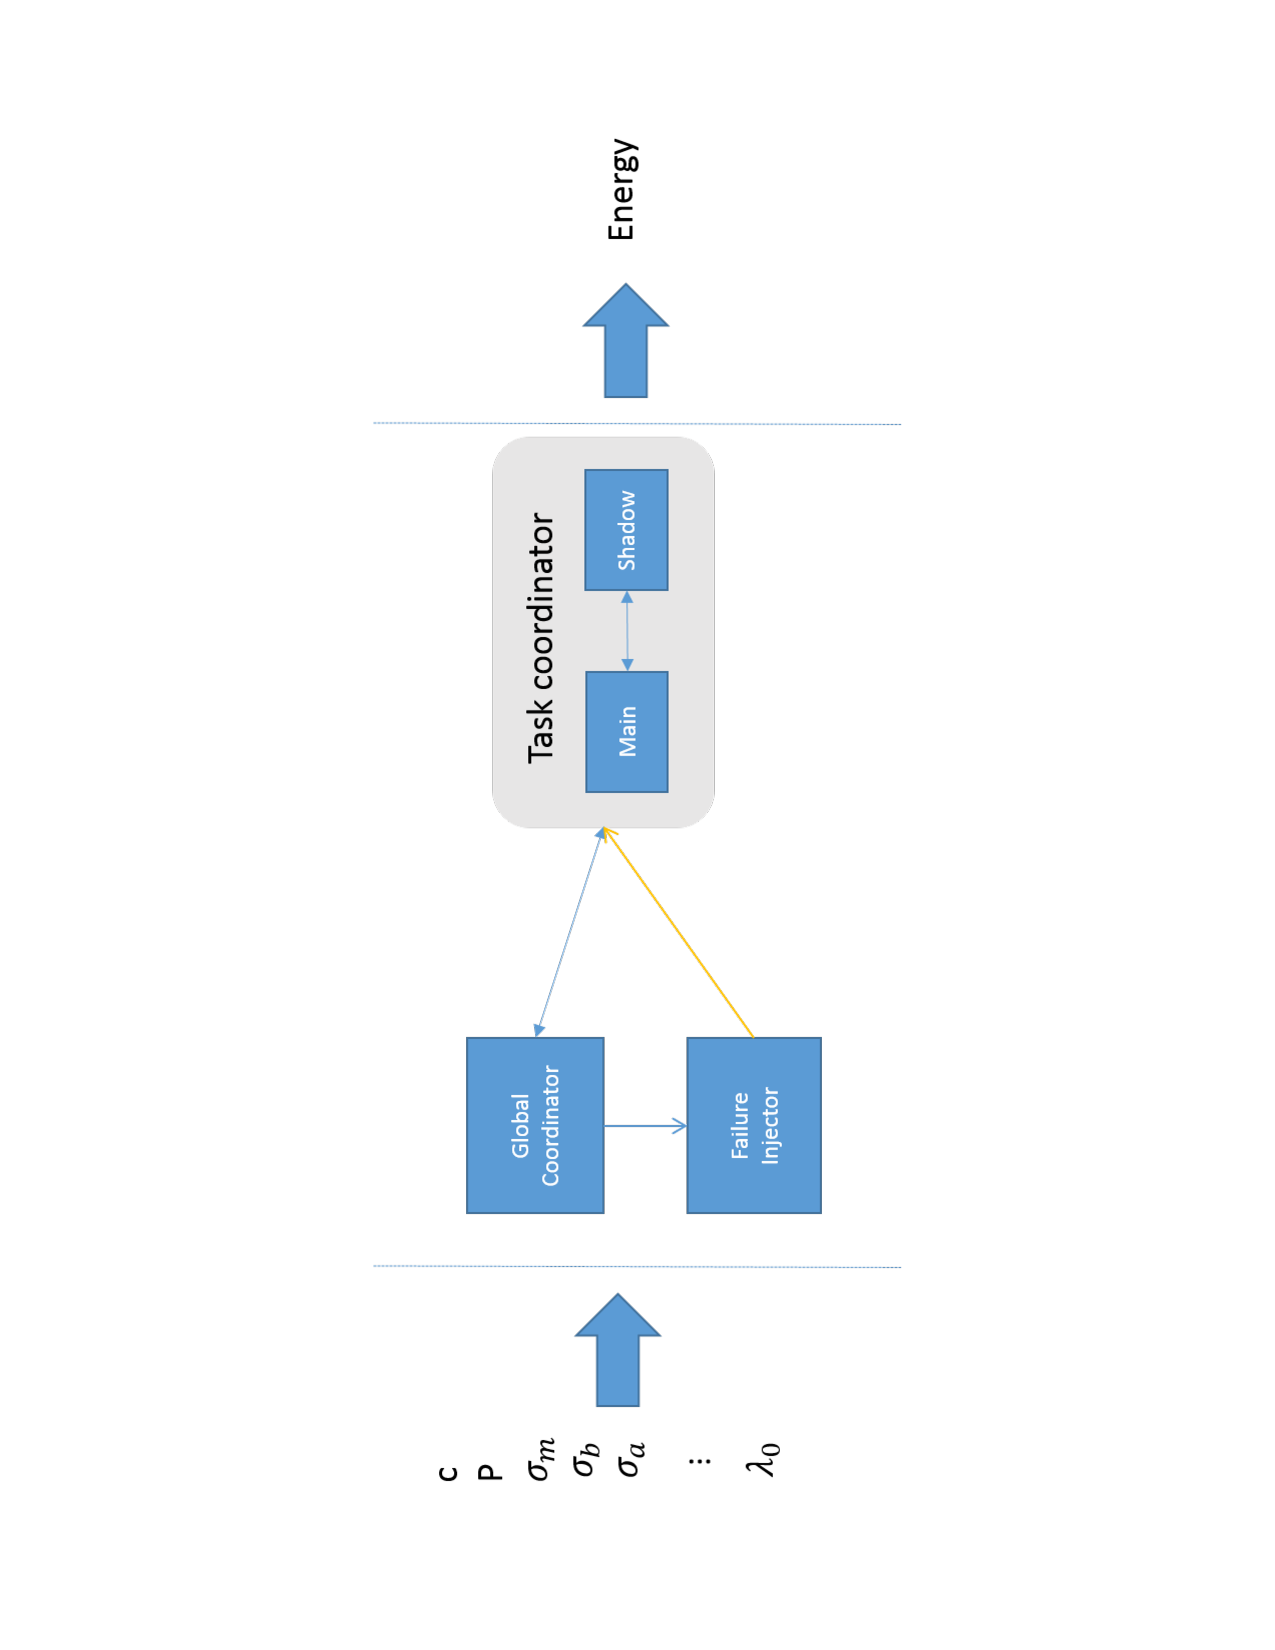
\includegraphics[width=0.5\columnwidth]{Figures/simulator}
	\end{center}
	\caption{Simulator architecture}
	\label{fig:sim}
\end{figure}

Using the simulator, we repeat the study for shadow replication as shown in Fig.~\ref{fig:failure_impact}  and Fig.~\ref{fig:utilization_impact}. 
The results obtained from our simulation are shown in Fig.~\ref{fig:comparison} as the orange lines, and the analytical results are shown as blue dotted lines. 
Each data point is the average of 20 runs. Due to the very low failure rate ($\lambda_0=10^{-6}$), we only see one failure during all the simulation runs. It is clear from Fig.~\ref{fig:comparison} that the results from simulation closely match our previous results from analytical models.

\begin{figure}[!t]
	\begin{center}
		\subfigure[Impact of target task failure probability]
		{
			\label{fig:com_failure}
			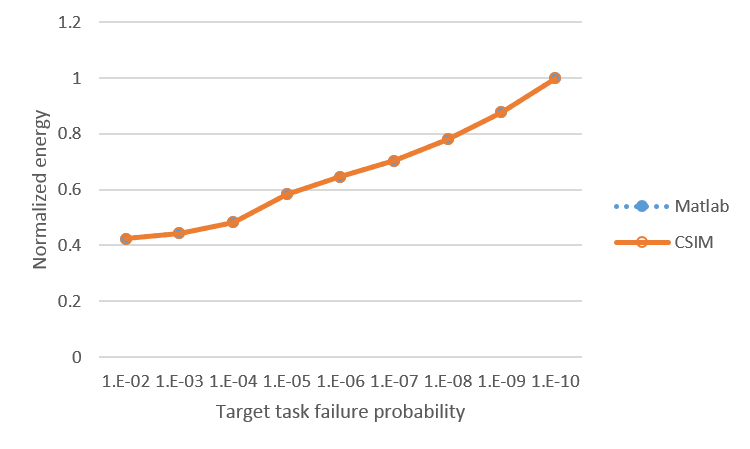
\includegraphics[width=0.45\columnwidth]{Figures/matlab_energy_vs_failure_10_100}
		} 
		\subfigure[Impact of utilization]
		{
			\label{fig:com_uti}
			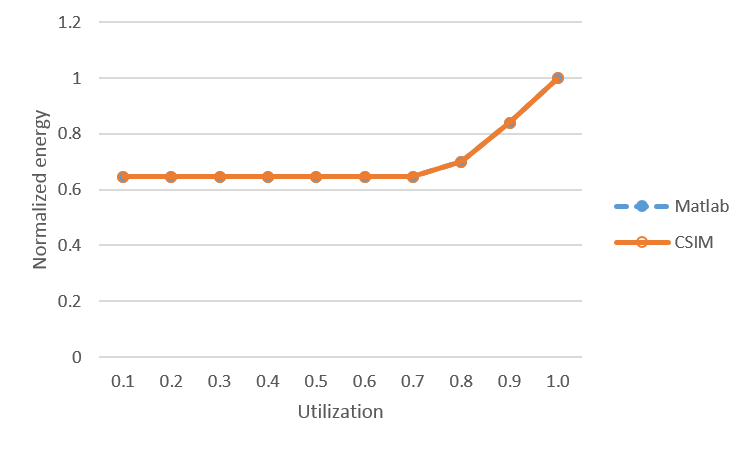
\includegraphics[width=0.45\columnwidth]{Figures/matlab_energy_vs_uti_10}
		} 
	\end{center}
	%\vskip -0.22in 
	\caption{Comparison between analytical and simulation results. $c=10ms$, $f_{min}=0.5$, $\alpha=0.1$, $d=4$, $\lambda_0=10^{-6}$.}
	\label{fig:comparison}
\end{figure}


